%                                   PREAMBLE

\documentclass[a4paper,10pt,twocolumn]{article}

\usepackage{amsthm}
\newtheorem{prop}{Proposition}
\theoremstyle{definition}
\newtheorem{defn}{Definition}

\usepackage{minted}

\usepackage{enumitem}
\usepackage{graphicx}

\usepackage{tikz}
\usetikzlibrary{arrows.meta, positioning, fit, patterns, shapes.geometric,
  shapes.multipart}

% Typographical tweaks
\usepackage{microtype}

% XXX Cursed settings
\usepackage[style=authoryear-icomp,maxcitenames=1,maxbibnames=999,uniquename=false,uniquelist=false]{biblatex}
%\usepackage{biblatex}
\addbibresource{report.bib}

\ifdefined\isdraftmode
  \usepackage{todonotes}
\else
  \usepackage[disable]{todonotes}
\fi

% Style taken from the ACM Primary Article template.
\usepackage{unicode-math}
\setmathfont[Scale=MatchUppercase]{LibertinusMath-Regular.otf}
\usepackage[tt=false]{libertine}
\setmonofont[StylisticSet=3]{inconsolata}

% Should be at the end, for some reason
\ifdefined\isdraftmode
  \usepackage[hidelinks]{hyperref}
\else
  \usepackage{hyperref}
\fi
\usepackage{cleveref}

\frenchspacing
\newcommand*{\code}{\texttt}
\newcommand*{\acronym}{\textsc}
\newcommand*{\IsabelleHOL}{Isabelle/\acronym{Hol}}
\newcommand*{\API}{\acronym{Api}}
\newcommand*{\WASM}{\acronym{Wasm}}

\newcommand*{\hoare}[3]{%
  \left\{\,{#1}\,\right\}
  \mathrel{#2}\nolinebreak
  \left\{\,{#3}\,\right\}
}
\DeclareMathOperator{\usage}{usage}
\DeclareMathOperator{\execscf}{exec\_scf}

%                                   DOCUMENT

\title{
  Exploiting Microarchitectural Timing Channels from JavaScript \\
  \acronym{Comp}6841 Project Report}
\author{Thomas Liang \\ z5418574 \\ \textsf{thomas.liang@unsw.edu.au}} % XXX

\begin{document}
\maketitle

\section{Project Description}

My project was to attempt to replicate a timing channel attack described by
\textcite{Oren_KSK_2015}, and to research and test possible improvements on
their attack method.
I will refer to this project as ``the paper'' or ``the attack'' for the rest of
this report.
I chose this project because it is tangentially related to my Honours thesis: I
am working at Trustworthy Systems\footnote{\url{https://trustworthy.systems/}},
as part of the work to show that the seL4
microkernel\footnote{\url{https://sel4.systems/}} is free of timing channels.

The attack I was replicating was a turning point in web security, as it showed
that JavaScript code executed in a browser context was able to detect the
behaviour of the rest of the browser and computer.
Merely by loading the website, a user could be attacked.
It did so by measuring and exploiting timing variations caused by the
\acronym{cpu} cache present in early Intel Core \acronym{cpu}s.

Because the source code for the attack is not public, there was no existing
reference code to draw from.
I needed to build a deep understanding of the attack from the paper and other
readings, and then continually experiment, measure, and iterate on my method.

I completed my project to limited success:
\begin{itemize}[nosep]
\item I demonstrated the presence of cache-based timing channels measurable
  inside JavaScript
\item I used Python and Matplotlib to analyse the exact effect of those timing
  channels
\item I applied my knowledge of systems programming, and data structures to
  optimise the performance of my implementation of the cache-profiling algorithm
\end{itemize}
For what it's worth, I also contacted the first author of the paper I am
referencing, Dr Yossef Oren, about my project asking for advice.
Part of our correspondence is presented in Appendix B.

However, other parts of my project had limited results:
\begin{itemize}[nosep]
\item My attempt to improve on their method by using WebAssembly failed, due to
  a mistake when checking browser compatibility.
\item My cache-profiling algorithm seems to work, but I could not optimise it
  enough to run in a feasible time for an attack.
\end{itemize}

Overall, this project taught me skills across a range of disciplines.
In particular, I want to emphasise that I learnt about:
\begin{itemize}[nosep]
  \item \acronym{Cpu} architecture, particularly how set-associative caches
work, which are used in all modern x86 Intel and \acronym{Amd} processors
  \item Optimising JavaScript code, by learning about the behaviour of
    \acronym{jit} compilers, and the internals of the Firefox JavaScript engine
    SpiderMonkey
  \item The history of browser security, the wide range of security mechanisms
    modern browsers contain, and why creating a sandbox is so difficult
\end{itemize}

In this report, I will briefly outline the technical basis for the attack and
its components, my experience replicating the attack, and ...
In the appendix, I include a link to the artifacts for my project, some of the
emails I exchanged with Dr Oren, and a rough timeline of my project.

\section{Background for the Attack}

Can a page loaded in a browser see what other websites you are visiting?
According to \textcite{Oren_KSK_2015}, the answer is yes.

Your web browser executes JavaScript (JS) code in an isolated environment that should
not be able to communicate outside its process, yet security researchers have
exploited Web \API{}s to leak information to and also to spy on the rest of your
machine.
JS abstracts away low-level details such as memory addresses and process
management, and has no \emph{explicit} mechanisms for communication with the
other browser tabs that are open, or processes running on the machine.
On paper, it should be safe to execute arbitrary JS code downloaded from
the websites you visit (and the vast majority of web users do so!).
However, the interface exposed by your browser (so-called Web \API{}s) are full
of \emph{side-channels}, from the time it takes to load videos, and for this
project, the time it takes to access a variable, which malicious code can
exploit to learn information.

In 2015, \textcite{Oren_KSK_2015} showed that by measuring the impact of cache
misses, JS code could accurately predict (1) what other websites the
browser had open on other tabs, and (2) hardware events, such as mouse activity,
and even the motion of a user in front of a laptop.
By using the High Resolution Time API, which could be used to measure time at a
nanosecond-resolution, they could determine what elements of a buffer were part
of the same \emph{cache set}.
By monitoring accesses to certain cache sets, the authors could determine a
unique memory-access ``fingerprint'' for different popular websites, and that
are triggered by hardware events.

According to Dr Oren in private correspondence, as a result of this paper and
other work, browser vendors quickly lowered the resolution of time that
JavaScript code had access to.

\section{Implementing the Attack}

My primary focus was on implementing Algorithm 1 from the paper, which is the
heuristic algorithm that finds an ``eviction set'' for a particular victim variable.
The eviction set is a set of offsets into the eviction buffer (16 offsets, for
the i7-6600U) that are in the same cache set as the victim.
Thus, by accessing each of those offsets, we can guarantee that the cache set is
\emph{primed}, and only contains values from addresses in the attacker's memory
allocation.

First, I sought out to measure the timing variation caused by cache misses
overall.
This is essential information for calibrating the cache-profiling algorithm.
Fortunately, I found \code{an4/Spy}\footnote{\url{https://github.com/an4/Spy}},
a GitHub repository containing the artifacts for Ana Dumitras' dissertation on a
web timing attack.
She cites \textcite{Oren_KSK_2015}, and provides some code to measure the timing
variations.
I adapted that code into my own style, rewriting it in TypeScript.

Next, I sought out to implement Algorithm 1.
The primary difficulty for this part was all the optimisations required.
I made a major error in that I skipped over Optimisation #1 listed in the paper,
which reduces the search space for the algorithm from over 131K offsets to just 8K.
Embarrassingly, I only discovered this in the final week of the project.
Other optimisations I learnt about are as follows:

\paragraph{Just-In-Time compilation.}
Because the JS engine in Firefox (and in most browsers) is a
Just-In-Time (\acronym{jit}) compiler, code gets faster the more it is run.
When code is run, the engine learns to perform more optimisations based on
what types each variable can hold, what fields objects have, etc.
This means that it is essential to run your benchmarking code at least a few
times to ``warm-up'' the code, to let the engine optimise it, for an
accurate measurement.

\paragraph{\code{var} versus \code{let} bindings.}
There are two ways of declaring mutable variable bindings in JS, with the
older \code{var} or newer \code{let} form.
A variable declared with \code{var} has scope of the surrounding function body,
whereas a \code{let} binding has scope the enclosing block.
An unfortunate consequence of this caused performance disparities in early
JavaScript engines including NodeJS, between \code{for} loops that used
\code{var} versus \code{let}.
If you used \code{let} to declare a variable in a \code{for}-loop, its scope was
just the loop body.
Unoptimised engines would then \emph{re-declare your variable on every
  iteration}.
Firefox 34 is so old that changing all my uses of \code{let} to \code{var}
caused a noticeable change in performance.
To be safe, all variables in hot loops are ``pre-allocated'', by being declared
but uninitialised prior to the loop.
This would be considered bad practise in modern software engineering, but
essential for this attack.

I learnt about SpiderMonkey internals from the official
documentation\footnote{\url{https://spidermonkey.dev/docs/}}.

\paragraph{Avoiding compiler optimisations}
Another minor issue is that in order to manipulate the cache into the state we
want, we need to do a lot of memory accesses.
However, we do not really do anything with the values returned by those
accesses.
To a clever compiler, those accesses are meaningless, and can be replaced in a
process called \emph{constant-folding}.
Thus, it's necessary to obfuscate your code in ways that the compiler does not
realise the accesses are pointless.
In Rust, this occurred as calls to \code{std::hint::black\_box}, a function for
writing benchmarks that tells the compiler to be ``maximally pessimistic'' about
what the function could possible do.
In the JS implementation, rather than doing a simple \code{for}-loop accessing
each field of the eviction buffer in turn, we turned the eviction buffer into
its own linked list.
Each value in the array ``pointed'' to the next element, and so we iterated
through the buffer as if we were traversing a linked list.

\paragraph{\WASM{} optimisation.}
Because of how abstract the JS runtime is, the algorithms outlined in
the paper are \emph{heuristics}, and so do not always succeed.
One reason is because the JavaScript runtime will also
touch the cache in unpredictable ways, interfering with our measurements.
I had a hunch that we might be able to lower this by running the measurements in
WebAssembly (\WASM{})\footnote{\url{https://webassembly.org/}}, a relatively-new
format for web programming language that is similar to native machine code.
The hope is that by using \WASM{} we can have maximum control over what the browser
does while executing the attack, and minimise cache interference.

To generate \WASM{} code, I chose to use Rust, a programming language that is
gaining popularity for low-level systems programming.
Rust was the natural choice for a few reasons:
it provides a type system that is explicit about casting between
integer sizes, which is essential for the tricky memory accesses our algorithms
do;
Rust is likely the language with the most comprehensive \WASM{} story after C/C++.
This required spending time learning how to set up a Rust and \WASM{} toolchain,
using libraries like \code{wasm-bindgen}.

\section{Results}

Here is a collection of things I learnt while trying to implement the project.

\subsection{Browser versioning is hard}

My attempt to implement the algorithm using Rust and \WASM{} failed because of
browser incompatibilities that I was unaware of.
I sourced all my information about what technologies and \API{}s a browser
version supported from Can I use...\footnote{\url{https://caniuse.com/}}, a free
online database about browser support.

The vulnerability identified by the paper depends on the High Resolution Time
API, which manifests as the function \code{Performance.now()}.
On Firefox 34, the version the authors demonstrated the attack on,
\code{Performance.now()} returned a timestamp with nanosecond-resolution.
This level of precision is essential to the attack.

The first version of Firefox to support \WASM{} is Firefox 52.
According to Can I use..., Firefox 15-54 is listed as supporting the High
Resolution Time API \parencite{caniuse}.
It seems that Firefox 52 would be the perfect attack target.
However, it turns out that Firefox 52 is a new enough version that the timer
resolution had already been silently lowered to mitigate timing-based attacks.
\footnote{I could not identify the exact version where this happened, but this
is verifiable by running Firefox 52 and checking the output of
\code{Performance.now}.}

This mistake cost me a lot of time working on an implementation in vain.
My Rust implementation can be seen in the \code{tc-spy-wasm} folder of the
artifacts respository.

\subsection{Silently priming the cache is hard}

The final obstacle that made my project unfeasible as an attack is because of
the necessity to \emph{prime} the cache.
An attacker primes the cache by accessing enough memory addresses to overwrite all parts
of the cache with its own memory.
That way, if another process changes the cache, the attacker can detect it by
the occurrence of a cache miss.

However, priming the cache can require thousands of memory accesses, even with
the optimisations listed by the authors.
Because old browsers are often single-threaded, which is supported by the
cooperative multithreading environment provided by JS, doing a lot of work on
the \acronym{cpu} can freeze the whole browser.
You can mitigate this by manually adding yield points to a hot loop.
On Firefox 34, the only way to do so is to use \code{setTimeout}, which will run
the provided callback function after a set number of milliseconds.
However, according to the HTML standard, the minimum passed timeout is 4 ms.
That means adding a yield point to a loop will incur a 4 ms penalty each time.
When we are measuring timing variations to the nearest nanosecond, one millionth
of a millisecond, that cost is an eternity.

When a script is taking up all the \code{cpu} of the process, browsers are
clever enough to ask the user if they would like to end the process.
That would stop my implementation of the attack in its tracks.

\appendix
\section{Project Timeline}

\begin{description}
\item[Week 3]
  I spent the week trying to acquire a machine to test my attack on.
  The authors demonstrated the attack on 2nd-5th generation Intel Core
  CPUs, and the algorithm they described relies on behaviour unique to the
  caches on Intel Core.
  I needed to find a machine with a CPU of a similarly old generation, such that
  its cache organisation had been reverse-engineered and made public online.
  Luckily, my partner had an old MacBook Pro with an Intel Core i7-6600U, which
  matched those requirements.
\item[Week 4]
  Trying to set up a VM.
  The paper demonstrates the attack on Ubuntu 14.04 running on VMWare Fusion 7.
  That version of Fusion is no longer officially available.
  The MacBook Pro I was testing my code on ran MacOS Big Sur, which was too old
  for the oldest available version of Fusion.
  The only other two hypervisor options were UTM or VirtualBox.
  I had various graphics incompatibilities with UTM and Ubuntu 14.04, so I had
  to use VirtualBox.
\item[Week 5]
  Implementing Rust version.
\item[Week 6]
  Reimplementing the JS version, using just what the paper describes.
\item [Week 7]
  Hopelessly trying to optimise the above implementation.
  Rewriting to have the various optimisations described above.
\item [Week 8]
  Writing this report.
\end{description}

\section{Correspondence with Dr Oren}

\begin{center}
  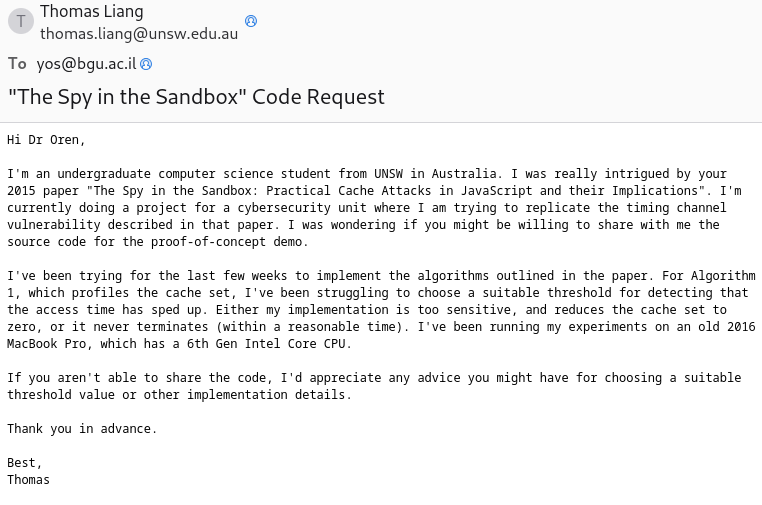
\includegraphics[width=0.5\textwidth]{email-to-oren.png}
  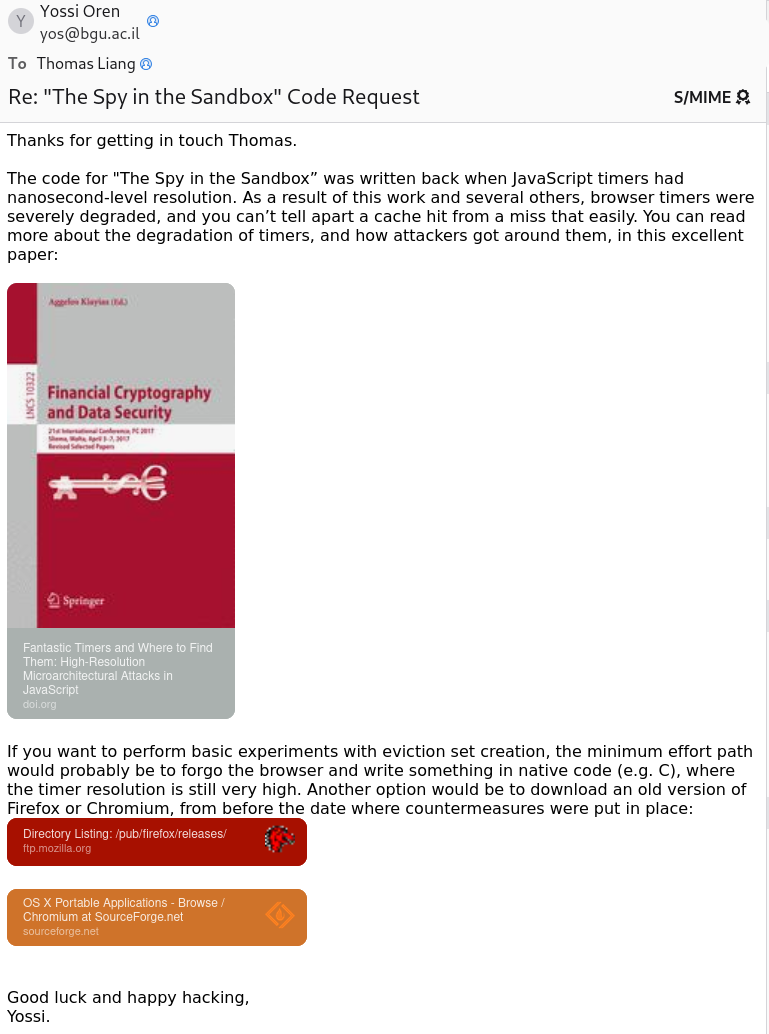
\includegraphics[width=0.5\textwidth]{reply-from-oren.png}
\end{center}

\section{Link to artifact}

You can find all the artifacts for this project at the following GitHub
repository: \url{https://github.com/ShunyaoLiang/comp6841-sap}.

\printbibliography



\end{document}
